\documentclass{article}
\usepackage{mainPoly}

\title{Variation instantanée, Variation globale}
\date{}
\author{Maths Spécifiques}

\begin{document}
\maketitle

\section{Variation instantanée}
\subsection{Introduction}
Deux voitures parcourent le même trajet sur la même route. Elles partent en même temps et mettent toutes deux le même temps pour arriver à destination. Les deux courbes ci-dessous représentent les kilomètres parcourrus en fonction du temps.

\begin{center}
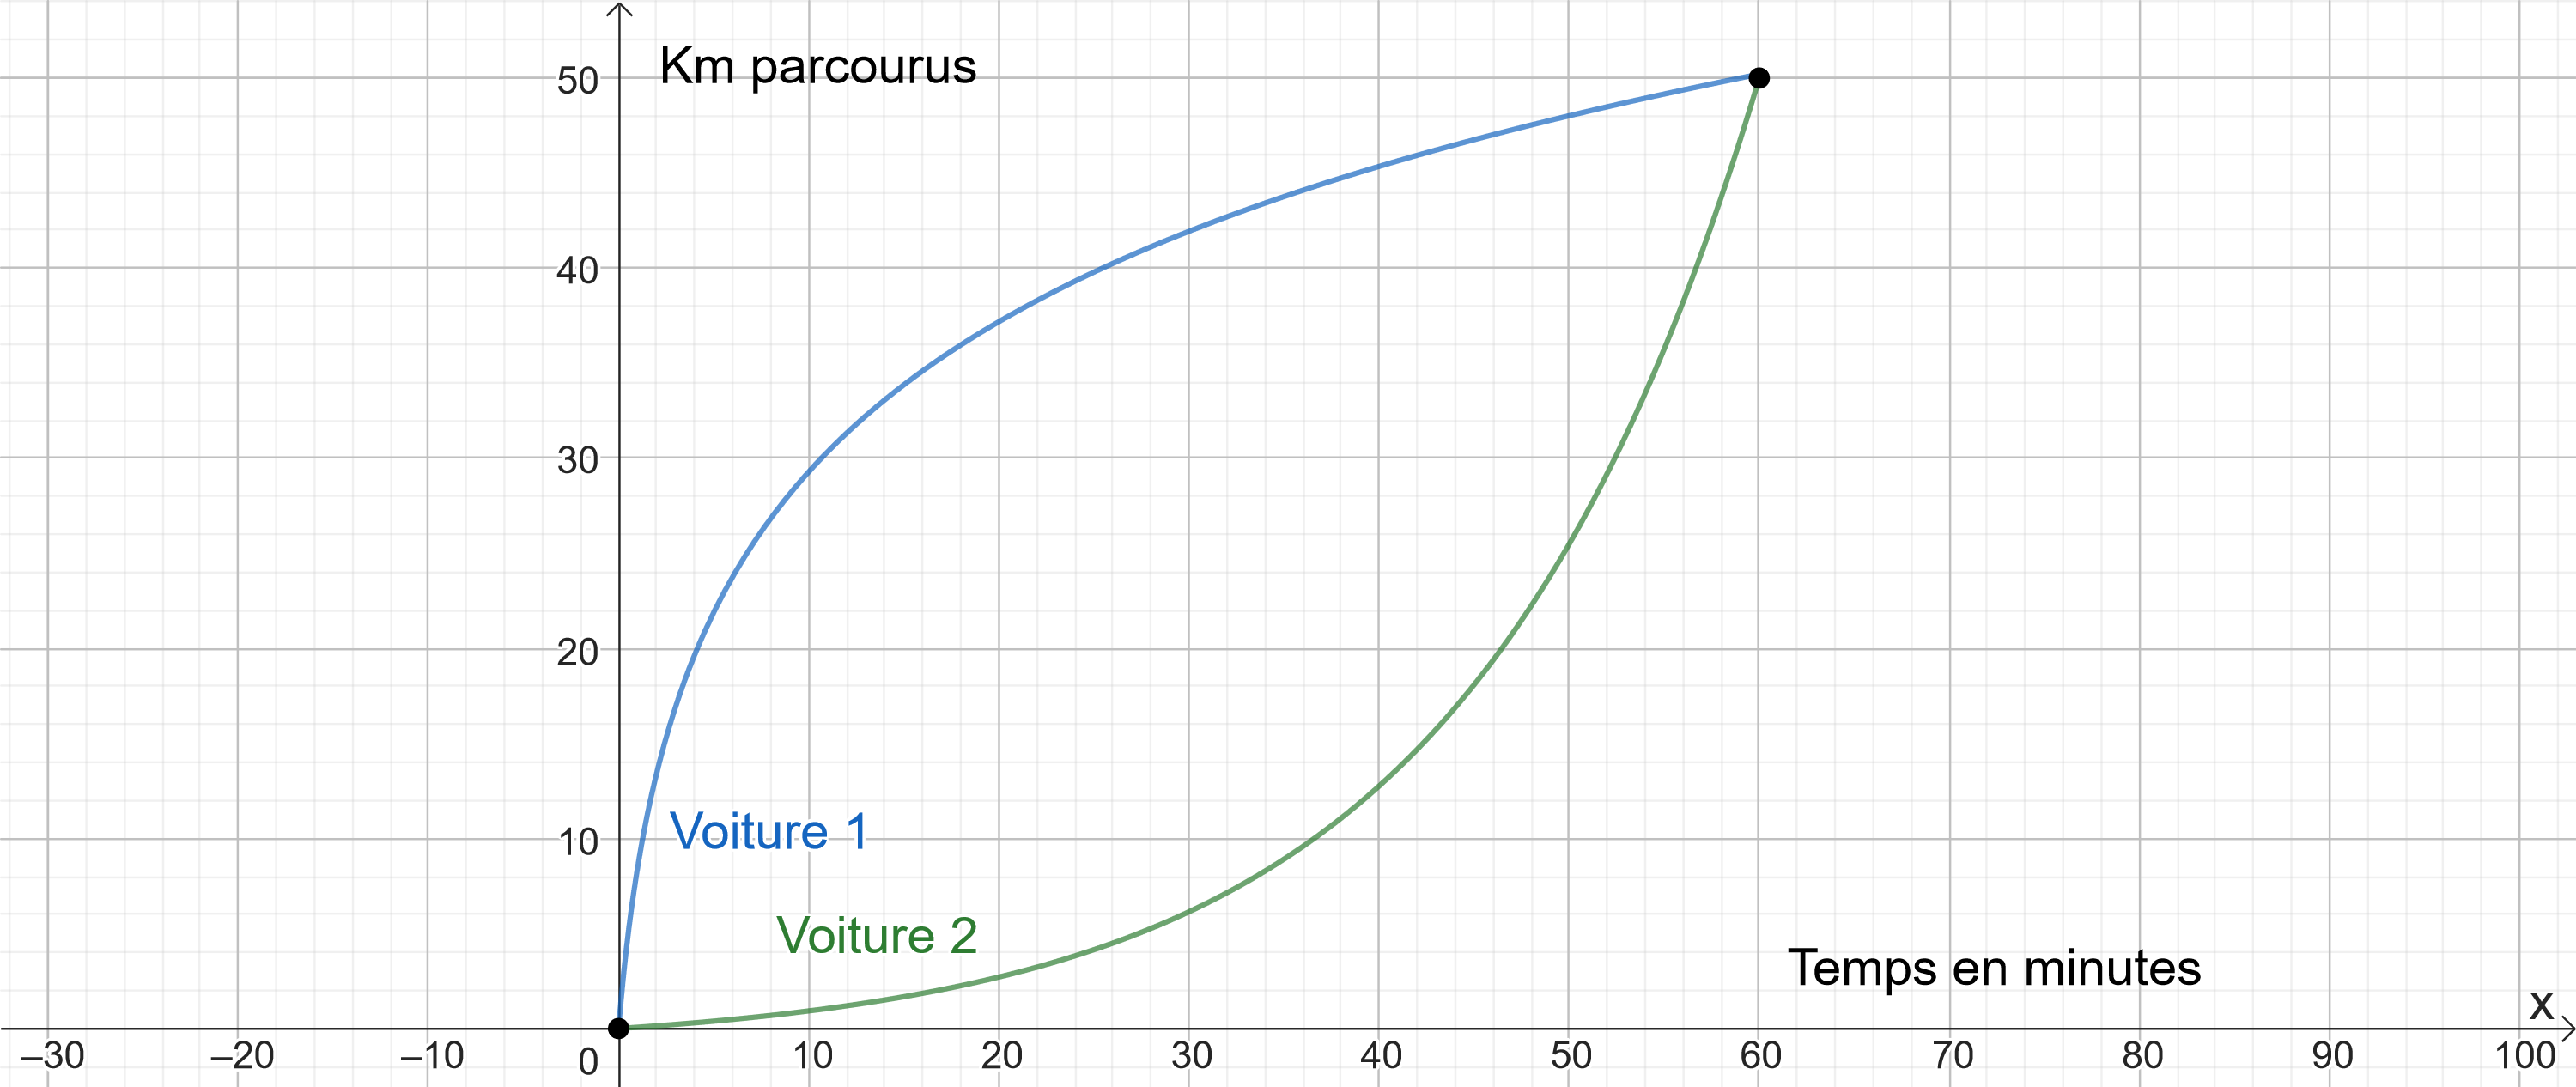
\includegraphics[width=0.9\textwidth]{Voitures.png}
\end{center}

\begin{exercize}
\begin{enumerate}[label=\emph{\alph*)}]
\item Quelle est la distance du trajet ? En combien de temps ces deux voitures ont-elles parcourru ce trajet ?
\item Quelle voiture allait plus vite sur les $30$ premières minutes ? Pourquoi ?
\item Admettons qu'une troisième voiture parcourt le trajet, mais garde la même vitesse du début à la fin. Quelle est cette vitesse en \unit{\kilo\meter\per\hour} ?
\item Combien de kilomètres a parcourru la voiture $1$ au bout de $30$ minutes ? Même question pour la voiture $2$.
\item Admettons qu'une quatrième voiture roule $30$ minutes et parcourt la même distance que la voiture $2$ au terme de ces $30$ minutes, mais en gardant une vitesse constante durant tout le trajet. Quelle est cette vitesse ?
\end{enumerate}
\end{exercize}
\emptybox{6cm}
\newpage
On trace les trajets des voitures $3$ et $4$ des questions précédentes. Leur vitesse constante est donnée par la \emph{pente} de la droite correspondante.
\begin{center}
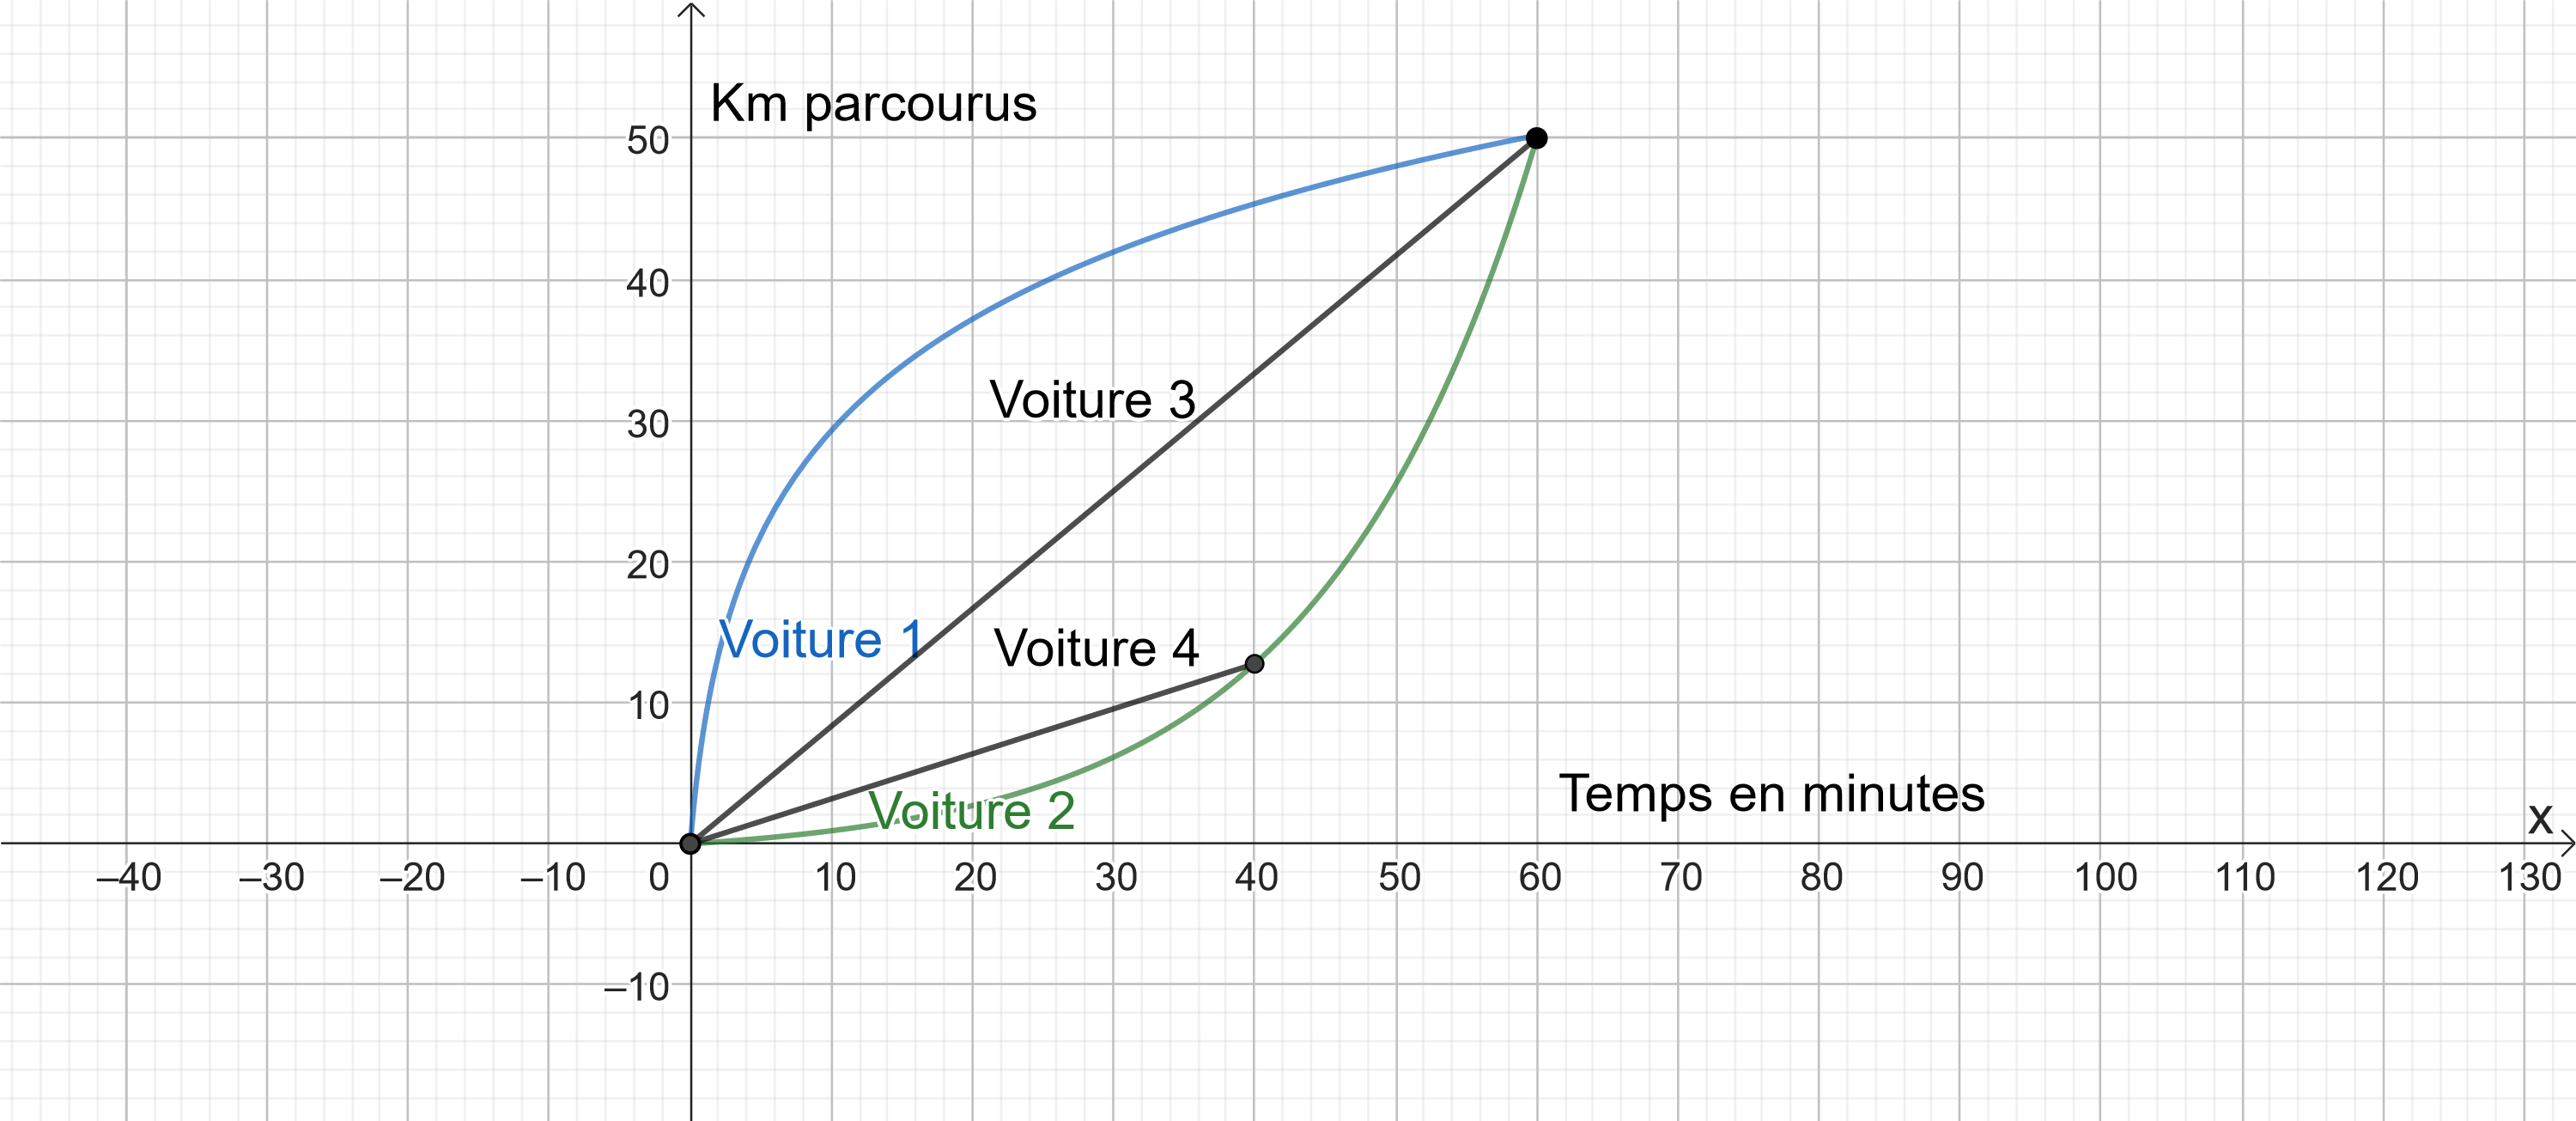
\includegraphics[width=0.9\textwidth]{Pentes.png}
\end{center}
S'il est facile d'estimer la vitesse d'une voiture dont la vitesse est constante, il est plus difficile de le faire dans le cas où une voiture a une vitesse variable. Pourtant, les compteurs de nos voitures estiment facilement la vitesse à laquelle nous roulons.

\begin{exercize}
Sur le schema suivant, faire figurer le trajet d'une voiture\dots
\begin{itemize}
\item Arrivant au bout de la $20$\ieme minute au même kilométrage que la voiture $2$
\item Arrivant au bout de la $40$\ieme minute au même kilométrage que la voiture $2$
\item Et roulant à vitesse constante entre la $20$\ieme et la $40$\ieme minute.
\end{itemize}
Quelle est la vitesse de la voiture entre $20$ et $40$ minutes ?
\end{exercize}
\begin{center}
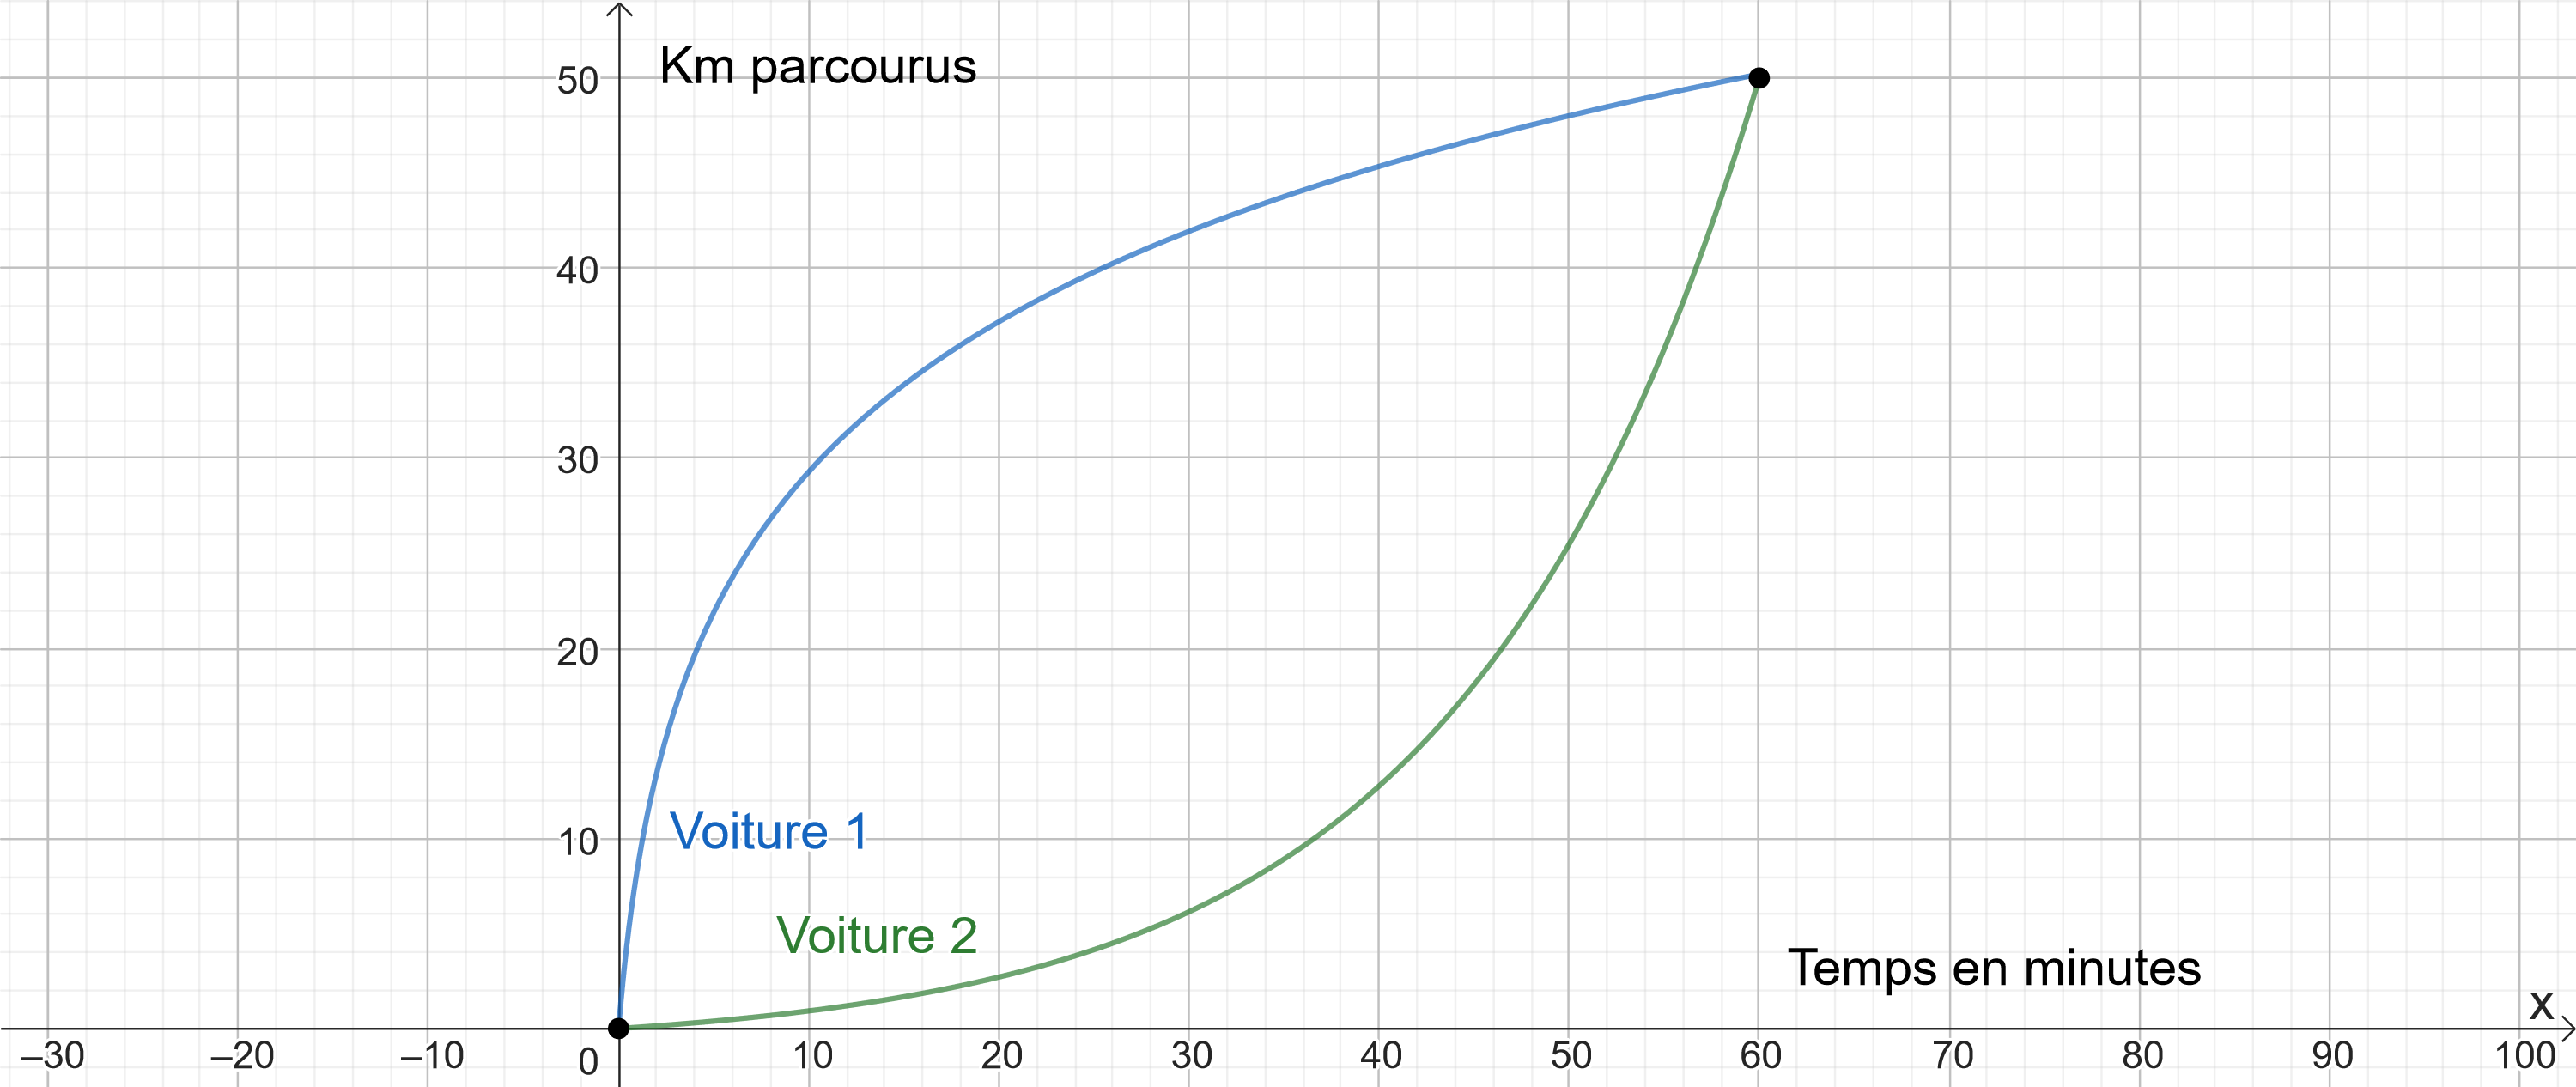
\includegraphics[width=0.9\textwidth]{Voitures.png}
\end{center}
\newpage
\subsection{Variation instantanée}
\begin{definition}
Soit $f : I \to \R$ une fonction dont la courbe représentative est donnée $\mathcal{C}_f$. Une droite est appelé \emph{sécante} à $\mathcal{C}_f$ si elle coupe deux points distincts de la courbe.
\end{definition}
\begin{center}
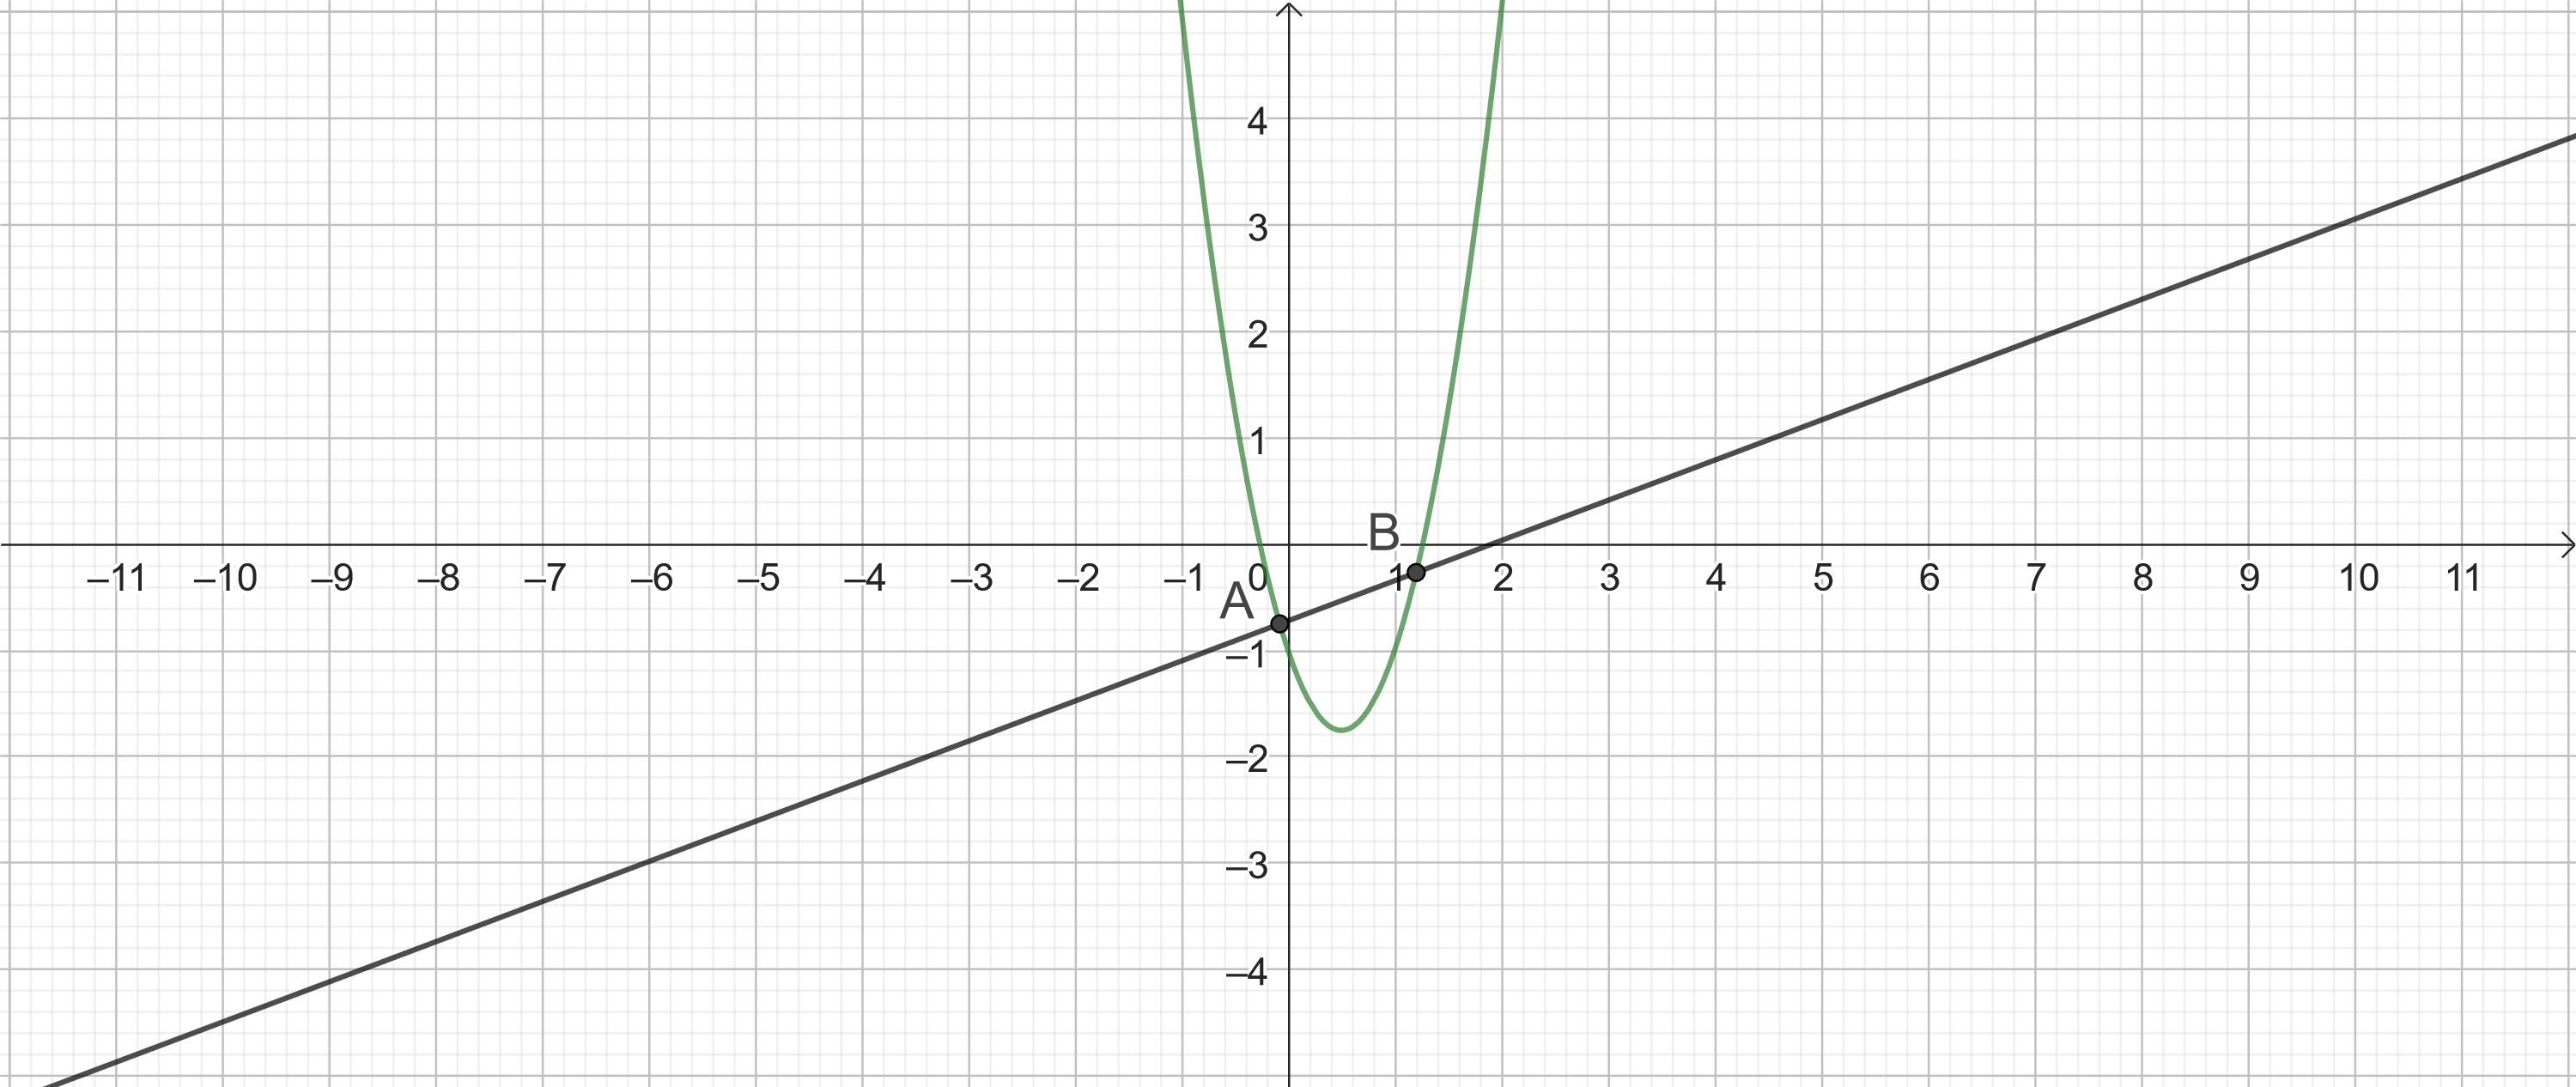
\includegraphics[width=0.9\textwidth]{Secante.png}    
\end{center}
\begin{remark}
\begin{itemize}
\item Une sécante à $\mathcal{C}_f$ ne peut pas être verticale.
\item \'Etant donné une sécante à $\mathcal{C}_f$, il existe une fonction affine $x \mapsto ax + b$ dont la courbe représentative est exactement cette sécante. 
\end{itemize}
\end{remark}
\begin{exercize}
Soit $f : I \to \R$ une fonction, et une sécante $d$ à $\mathcal{C}_f$.
\begin{enumerate}[label=\emph{\alph*)}]
\item Justifier que $d$ passe par deux points de la forme $(x_1;f(x_1))$ et $(x_2;f(x_2))$ avec $x_1,x_2 \in I$.
\item Soit $g:x \mapsto ax + b$ une fonction affine dont la courbe représentative est $d$. Justifier que sa pente vaut
\begin{equation*}
a = \dfrac{f(x_1)-f(x_2)}{x_1-x_2}    
\end{equation*}  
\end{enumerate} 
\end{exercize}
\emptybox{3cm}
\begin{tcolorbox}
On suppose que $A(x_1;f(x_1))$ est fixé. Plus $B(x_2;f(x_2))$ est proche de $A$, plus la sécante à $\mathcal{C}_f$ passant par $A$ et $B$ se rapproche d'une position limite. Cette droite limite est appelée \emph{tangente} à la courbe $\mathcal{C}_f$ passant par $A$. 
\end{tcolorbox}
\begin{remark}
Quand elle existe, la tangente à la courbe $\mathcal{C}_f$ est unique.
\end{remark}
\begin{definitionbox}
Soit $f : I \to \R$ une fonction, et $a \in I$. On appelle nombre dérivé de $f$ en $a$ la pente de la tangente à $C_f$ passant par $A(a;f(a))$.
\end{definitionbox}
\begin{remark}
Pour calculer le nombre dérivé de $f$ en $a$, on regarde vers quelle valeur le taux d'accroissement
\begin{equation*}
\dfrac{f(a)-f(x)}{a-x}    
\end{equation*}
se dirige quand $x$ se rapproche de $a$.
\end{remark}
\newpage
\section{Variation globale}
\subsection{Fonction dérivée}
\begin{definitionbox}
Soit $f$ un fonction définie sur un intervalle $I$ et admettant un nombre dérivé sur tout $a$ appartenant à $I$. On dit que $f$ est dérivable sur $I$.
\end{definitionbox}
\begin{definitionbox}
Soit $f$ une fonction définie sur un intervalle $I$ et dérivable sur $I$. Alors on note $f'$ la fonction définie sur $I$ qui a tout nombre $a$ dans $I$ associe le nombre dérivé de $f$ en $a$. 
\end{definitionbox}
\begin{remark}
\begin{itemize}
\item Pour parler de la fonction dérivée de $f$, il faut avoir préalablement dit que $f$ est dérivable. 
\end{itemize}
\end{remark}
\begin{example}
\begin{enumerate}
\item Soit $f \colon x \mapsto \dfrac{1}{2}x+1$ définie sur $\R$. La fonction $f$ admet un nombre dérivé en $a$, pour n'importe quel $a$ appartenant à $\R$. Ce nombre dérivé est toujours $\dfrac{1}{2}$. On en déduit que la \emph{fonction dérivée} de $f$, $f'$, est la fonction telle que pour tout $a$
\begin{equation*}
f'(a)=\dfrac{1}{2}\,.
\end{equation*} 
\item Soit $g \colon x \mapsto x^2$ définie sur $\R$. La fonction $g$ admet un nombre dérivé en $a$, pour n'importe quel $a$ appartenant à $\R$. On en déduit que $g$ est dérivable sur $\R$. La fonction dérivée de $g$, $g'$, est la fonction définie sur $\R$ et telle que
\begin{equation*}
g'(x)=2x
\end{equation*}
\end{enumerate}
\end{example}
\begin{tcolorbox}
\begin{proposition}
Soit $f$ une fonction définie sur $I$ et dérivable sur $I$. Soit $J$ un intervalle inclus dans $I$. Alors,
\begin{itemize}
\item $f$ est croissante sur $J$ si et seulement si $f'$ est positive sur $J$.
\item $f$ est décroissante sur $J$ si et seulement si $f'$ est négative sur $J$.
\end{itemize}
\end{proposition}
\end{tcolorbox}
\begin{example}
\begin{enumerate}[label=\emph{\alph*)}]
\item Soit $g \colon x \mapsto x^2$ définie sur $\R$. Pour quelles valeurs de $x$ a-t-on $g'(x) \geq 0$ ? Et $g'(x) \leq 0$ ?

\emptybox{2cm}
\item Compléter le tableau de variations suivant.
\begin{center}
\begin{tikzpicture}
\tkzTabInit{$x$/0.5, Signe de $g'$/2, Variations de $g$/2}{$-\infty$, $0$, $+\infty$};
\tkzTabLine{,,z,,};
\end{tikzpicture}
\end{center}
\end{enumerate}
\end{example}
\newpage
\subsection{Calcul de la fonction dérivée}
\begin{proposition}[Fonctions usuelles]
\begin{itemize}
\item Soit la fonction $f \colon x \mapsto 1$ définie sur $\R$. Alors cette fonction est dérivable sur $\R$ et sa dérivée $f'$ vérifie
\begin{equation*}
f'(x)=0
\end{equation*}
pour tout $x \in \R$.
\item Soit la fonction $f \colon x \mapsto x$ définie sur $\R$. Alors cette fonction est dérivable sur $\R$ et sa dérivée $f'$ vérifie
\begin{equation*}
f'(x)=1
\end{equation*}
pour tout $x \in \R$.
\item Soit la fonction $f \colon x \mapsto x^2$ définie sur $\R$. Alors cette fonction est dérivable sur $\R$ et sa dérivée $f'$ vérifie
\begin{equation*}
f'(x)=2x
\end{equation*}
pour tout $x \in \R$.
\item Soit la fonction $f \colon x \mapsto x^3$ définie sur $\R$. Alors cette fonction est dérivable sur $\R$ et sa dérivée $f'$ vérifie
\begin{equation*}
f'(x)=3x^2
\end{equation*}
pour tout $x \in \R$.
\end{itemize}
\end{proposition}
\begin{tcolorbox}
\begin{remark}
Pour l'écrire de façon condensée, on peut utiliser $\dv{x}(f(x))$. Donc,
\begin{equation*}
\begin{array}{cccc}
\dv{x}(1)=0; & \dv{x}(x)=1; & \dv{x}(x^2)=2x; & \dv{x}(x^3) = 3x^2
\end{array}
\end{equation*}
\end{remark}
\end{tcolorbox}
\begin{proposition}[Somme et produit par un réel]
Soit $f$ et $g$ deux fonctions définies et dérivables sur $\R$.
\begin{itemize}
\item Soit $k \in \R$, la fonction $h \colon x \mapsto k \times f(x)$ est alors dérivable sur $\R$. Et sa dérivée $h'$ vérifie
\begin{equation*}
h'(x) = k \times f'(x)
\end{equation*}
pour tout $x \in \R$.
\item La fonction $s \colon x \mapsto f(x) + g(x)$ est alors dérivable sur $\R$. Et sa dérivée $s'$ vérifie
\begin{equation*}
s'(x) = f'(x) + g'(x)
\end{equation*}
pour tout $x \in \R$.
\end{itemize}
\end{proposition}
\begin{tcolorbox}
\begin{remark}
\begin{equation*}
\begin{array}{cc}
\dv{x}(kf(x)) = k\dv{x}(f(x)); & \dv{x}(f(x)+g(x)) = \dv{x}(f(x)) + \dv{x}(g(x))
\end{array}
\end{equation*}
\end{remark}
\end{tcolorbox}
\begin{example}
Soit $f \colon x \mapsto 2x^3 + 3x^2 + 4x + 5$ définie sur $\R$. Justifier que $f$ est dérivable sur $\R$ et donner l'expression de sa dérivée.
\begin{tcolorbox}
$f$ est dérivable sur $\R$ en tant que somme de fonctions qui le sont.

Pour calculer sa dérivée $f'$, on utilise $\dv{x}(f(x))$.
\begin{equation*}
\begin{aligned}
\dv{x}(f(x)) &= \dv{x}(2x^3 + 3x^2 + 4x + 5)\\
&= \dv{x}(2x^3) + \dv{x}(3x^2) + \dv{x}(4x) + \dv{x}(5)\\
&= 2\dv{x}(x^3) + 3\dv{x}(x^2) + 4\dv{x}(x) + 5\dv{x}(1)\\
&= 2 \times 3x^2 + 3 \times 2x + 4 \times 1 + 5 \times 0\\
&= 6x^2 + 6x + 4
\end{aligned}
\end{equation*}
Donc la dérivée de $f$ est donnée par $f' \colon x \mapsto 6x^2 + 6x + 4$.
\end{tcolorbox}
\end{example}
\end{document}